% Overleaf: XeLaTeX. Main file = main_zh.tex (Chinese) or main_en.tex (English).
\documentclass[10pt,journal,compsoc]{IEEEtran}
\usepackage[UTF8,heading=false,fontset=fandol]{ctex}
\setmainfont{texgyrepagella-regular.otf}[BoldFont=texgyrepagella-bold.otf,ItalicFont=texgyrepagella-italic.otf,BoldItalicFont=texgyrepagella-bolditalic.otf]
\setsansfont{texgyreheros-regular.otf}[BoldFont=texgyreheros-bold.otf,ItalicFont=texgyreheros-italic.otf,BoldItalicFont=texgyreheros-bolditalic.otf]
\setmonofont{lmmono10-regular.otf}
\usepackage{amsmath,amssymb,amsthm,graphicx,booktabs}
\usepackage{algorithm,algpseudocode,cite}
\usepackage[hidelinks]{hyperref}
\newtheorem{theorem}{定理}
\renewcommand{\proofname}{证明}
\renewcommand{\abstractname}{摘要}
\renewcommand{\IEEEkeywordsname}{关键词}
\renewcommand{\refname}{参考文献}
\floatname{algorithm}{算法}
\algrenewcommand\algorithmicrequire{\textbf{输入：}}
\algrenewcommand\algorithmicensure{\textbf{输出：}}
\graphicspath{{figures/}}
\newcommand{\NaiveSmall}{0.3963}
\newcommand{\SlideSmall}{0.0310}
\newcommand{\NaiveMedium}{2.8641}
\newcommand{\SlideMedium}{0.0975}
\newcommand{\NaiveLarge}{31.3657}
\newcommand{\SlideLarge}{0.3098}

\begin{document}
\title{面向长语音检索的转写引导\\滑动窗口片段选择}
\author{作者姓名（提交前填写）\thanks{算法课程论文。实验使用公开 SPIRAL 转写标注，评估关键句检索。}}
\markboth{算法设计与分析课程论文}{转写引导的滑动窗口片段选择}
\IEEEtitleabstractindextext{%
\begin{abstract}
长录音中的目标信息通常位于局部片段，片段选择因而成为长语音检索的一个基本问题。本文受 SpeechPrune 的相关信息筛选思路启发，研究一种适合独立实现的转写引导方案：先用问题与转写句子的 TF-IDF 余弦相似度生成相关分数，再选择分数总和最大的固定句数连续窗口。通过维护窗口分数，算法在分数已知时以 $O(N)$ 时间和 $O(1)$ 额外工作空间求得最优窗口。本文给出循环不变式证明，并在 SPIRAL 全部 1,012 条转写标注上，与开头裁剪、随机窗口和分数 Top-$k$ 比较。在名义 20\% 句数预算下，滑动窗口的完整关键句跨度命中率为 86.86\%，随机窗口为 25.30\%，Top-$k$ 为 87.06\%；滑动窗口固定保留一个连续段，Top-$k$ 平均保留 2.68 段。在 50\% 预算下，两者命中率分别为 96.44\% 和 94.37\%。结果展示了连续性约束与检索覆盖率之间随预算变化的关系。实验评价的是基于已提供转写的关键句保留能力，预算单位为句子数。
\end{abstract}
\begin{IEEEkeywords}
长语音检索；滑动窗口；连续片段选择；TF-IDF；SPIRAL；算法分析
\end{IEEEkeywords}}
\maketitle
\IEEEdisplaynontitleabstractindextext
\IEEEpeerreviewmaketitle

\section{引言}
从会议、讲座和日常对话中找到与问题有关的内容，是长语音理解中的常见需求。例如，用户询问某次会议的具体时间，答案可能只出现于整段录音中的一句话。语音信息检索任务将这一需求表述为：给定长语音和一个问题，定位能够支持回答的信息。SpeechPrune 提出了相应任务与 SPIRAL 数据集，并通过筛选音频 token 降低后续处理规模\cite{lin2025speechprune}。

片段选择需要兼顾相关性与上下文连续性。按分数单独挑选若干位置能够获得较高的总相关分数，却可能形成多个分散片段；连续裁剪则保留一个区间内的原始顺序。本文围绕这个选择问题，采用容易检查的算法结构：给每个转写句子打分，然后用固定长度窗口沿句子序列扫描。

本文的研究问题是：\emph{在相同句数预算下，最大分数连续窗口能够保留多少标注关键句，与分散 Top-$k$ 选择有何差异？}为单独研究选择算法，本文直接使用 SPIRAL 已提供的转写句子，以词语匹配得到相关分数，随后评价被选句子是否覆盖标注关键跨度。问题文本用于打分，正确答案、选项与关键句位置均不参与分数计算。

本文给出固定长度最大和窗口的线性算法与正确性证明，在 1,012 条公开标注上比较四种选择规则，并通过标注审计和穷举扫描核对实现。TF-IDF 和滑动窗口均为已有技术，本文重点分析连续选择的计算过程与关键证据覆盖情况。

\section{相关研究}
\subsection{长语音理解与相关信息筛选}
Qwen2-Audio 等音频语言模型能够结合声音与文本指令执行分析任务\cite{chu2024qwen}。SpeechPrune 使用音频与问题文本的相似度进行初步筛选，再根据近似注意力分数进一步选择音频 token\cite{lin2025speechprune}。其实现已经包含分帧与时间结构的考虑。本文将这个问题简化为转写句子上的连续区间选择，以便解释每一步计算和验证输出。

时间邻近性也是音频表示压缩的已有研究因素。Luo 等在局部时间窗口内合并相近音频 token，并观察到局部性效果随任务变化\cite{luo2026locality}。这为比较连续与分散选择提供了相关背景；本文在句子层面单独考察两者的关键证据覆盖情况。

\subsection{转写检索与窗口选择}
语音识别系统可以将录音转换为文本，Whisper 是这一环节的代表研究\cite{radford2023whisper}。获得转写后，词项加权与向量相似度可以用于问题相关片段排序\cite{manning2008ir}。本文使用已提供的参考转写，避免把识别错误与选择错误混合在同一个实验中。

窗口和的最优性与关键句覆盖是两个评价层次，分别通过理论证明和数据实验检验。

\section{问题定义与相关度计算}
\subsection{输入、预算与目标}
设转写句子按录音顺序排列为 $X=(x_1,\ldots,x_N)$，问题为 $q$，句子相关分数为 $s_1,\ldots,s_N$。预算 $k$ 表示保留的句子数量，满足 $1\le k\le N$。从位置 $t$ 开始的连续窗口为
\begin{equation}
 W_t=\{t,t+1,\ldots,t+k-1\},\quad 1\le t\le N-k+1.
\end{equation}
本文选择总相关分数最大的窗口：
\begin{equation}
 t^*=\arg\max_t F(t),\qquad F(t)=\sum_{i=t}^{t+k-1}s_i.
 \label{eq:target}
\end{equation}
分数相同时，数学定义中选择开始位置最早的窗口。因为所有候选包含相同数量的句子，最大化总分也等价于最大化平均分。

本文预算统一为句子数量。不同句子的长度和说话时长可以不同，因此相同 $k$ 不表示相同秒数或相同音频 token 数。实验同时记录保留的文本词数比例，以显示这一差别。

\subsection{无需训练的句子打分}
本文采用 TF-IDF 加权与余弦相似度\cite{manning2008ir}。每条录音独立构造词表和文档频率，将该录音的各句子视为文档。设词 $v$ 出现在 $\mathrm{df}(v)$ 个句子中，使用平滑权重
\begin{equation}
 \mathrm{idf}(v)=1+\log\frac{N+1}{\mathrm{df}(v)+1}.
\end{equation}
词 $v$ 在文本 $x$ 中出现 $c(v,x)>0$ 次时，赋权
\begin{equation}
 z_v(x)=[1+\log c(v,x)]\,\mathrm{idf}(v).
\end{equation}
将句子向量和问题向量分别进行 $\ell_2$ 归一化，得到
\begin{equation}
 s_i=\frac{z(x_i)^\top z(q)}{\|z(x_i)\|_2\|z(q)\|_2}.
 \label{eq:score}
\end{equation}
零向量的相似度定义为 0。文本处理包括小写化、按字母词和数字切分，以及删除随代码固定提供的停用词；不使用词干化或语义模型。问题中没有在当前转写出现的词从本地词表中移除。完整规则在代码中固定，四种选择方法共用相同的分数。

\section{滑动窗口算法与理论分析}
\subsection{更新规则与实例}
直接枚举每个窗口并重新求和，需要 $O((N-k+1)k)$ 时间。相邻窗口包含 $k-1$ 个相同元素，可以复用这些计算：
\begin{equation}
 F(t+1)=F(t)-s_t+s_{t+k}.
 \label{eq:update}
\end{equation}
因此，只需计算第一个窗口的和，再反复减去离开的分数、加上进入的分数。

例如，分数序列为 $(1,2,8,9,7,1)$，窗口大小 $k=3$，四个窗口的和依次为 11、19、24、17。算法返回第 3--5 个位置，最大和为 24。该示例用于说明更新步骤，与数据集实验分开。

\begin{algorithm}[t]
\caption{固定句数最大分数窗口}\label{alg:window}
\begin{algorithmic}[1]
\Require 分数数组 $s_1,\ldots,s_N$，预算 $k$
\Ensure 最佳窗口开始位置 $t^*$ 与窗口和 $b$
\State 检查 $1\le k\le N$
\State $c\gets\sum_{i=1}^{k}s_i$；$b\gets c$；$t^*\gets1$
\For{$t=2,\ldots,N-k+1$}
 \State $c\gets c-s_{t-1}+s_{t+k-1}$
 \If{$c>b$}
  \State $b\gets c$；$t^*\gets t$
 \EndIf
\EndFor
\State \Return $(t^*,b)$
\end{algorithmic}
\end{algorithm}

\subsection{正确性证明}
\begin{theorem}
在精确算术下，算法~\ref{alg:window} 返回式~\eqref{eq:target} 的最优窗口；存在多个最优窗口时，返回开始位置最早的一个。
\end{theorem}
\begin{proof}
维护两个循环不变式：处理窗口 $t$ 后，变量 $c$ 等于 $F(t)$；变量 $b$ 等于已经处理的所有窗口中的最大和，$t^*$ 为其中最早的最佳开始位置。

初始化直接求出第一个窗口和，不变式成立。由式~\eqref{eq:update}，一次更新后，$c$ 恰好等于下一个窗口的和。若新窗口和更大，算法更新 $b$ 与 $t^*$；否则保留已有记录。严格大于的比较使平局保留更早的位置，因此两个不变式均保持。

终止时，所有 $N-k+1$ 个合法窗口都已处理，$b$ 就是全局最大窗口和，$t^*$ 满足所需的平局规则。
\end{proof}

\subsection{复杂度与实现边界}
第一个窗口求和耗时 $O(k)$，之后执行 $N-k$ 次常数时间更新，所以总时间为 $O(N)$。算法维护当前和、最大和、最佳位置等常数个变量，额外工作空间为 $O(1)$，不计输入分数数组与输出句子。参考代码通过逐项读取分数初始化，不额外复制长度为 $k$ 的子数组。

TF-IDF 特征构建和文本读取在窗口选择之前执行，其开销由词数与词表大小决定。本文的 $O(N)$ 结论针对分数已知后的选择步骤。实测计时也采用这一边界，单独比较朴素扫描与滑动更新。

当 $k=1$ 时，算法选择分数最高的一句；当 $k=N$ 时，返回整个转写。初始化使用第一个合法窗口，因此同样适用于全为负数的分数序列。实验分数非负，而正确性证明无需这一条件。

\section{实验设计}
\subsection{数据与标注审计}
实验使用 SPIRAL 公布的全部 1,012 条记录\cite{lin2025speechprune}，包括 350 条讲座、324 条会议和 338 条日常对话。SPIRAL 采用合成对话与语音，本文使用其中的参考转写、问题和关键句跨度。

本文采用 \texttt{audio\_data.combined.sentences} 中的句子顺序，并将关键句的 \texttt{indices} 按零起始、右端不包含的区间解释。所有 1,012 个区间均满足边界条件。句数最少为 6、最多为 34，平均为 17.06；891 条记录的关键跨度包含一句，121 条包含两句。

标注文本核对发现：924 条区间内文本与原始关键句规范化后完全一致，79 条包含原始关键句但有额外文本，9 条不属于这两类。主实验保留全部记录并沿用发布者的跨度标注；另报告 924 条完全一致记录上的敏感性结果，不人工移动标注位置。

\subsection{预算与比较方法}
对每条记录设置名义比例 $\rho\in\{0.1,0.2,0.3,0.5\}$，预算为 $k=\lceil\rho N\rceil$。四种方法保留相同数量的句子：开头裁剪保留前 $k$ 句；随机窗口在所有连续窗口开始位置上均匀采样；分数 Top-$k$ 选择相关分数最高的 $k$ 句并保留原始顺序；滑动窗口选择式~\eqref{eq:target} 的最佳连续窗口。

随机窗口的指标通过枚举所有合法开始位置计算精确期望，避免随机种子造成结果波动。Top-$k$ 在分数平局时选择更早的句子。全部预算预先固定，不使用正确答案或关键位置调参。

\subsection{评价指标}
设标注关键句集合为 $G$，选中句子集合为 $S$，主要指标为完整跨度命中率：
\begin{equation}
 H=\frac{1}{M}\sum_{j=1}^{M}\mathbf{1}[G_j\subseteq S_j],
\end{equation}
其中 $M=1012$。随机窗口用每条记录上的期望命中概率参与平均。另记录部分命中率、关键句召回率、所选分数之和以及连续片段数量。片段数量按相邻句子索引是否连续计算。

句数保留率为 $k/N$；词数保留率为所选句子分词后的词数占整条转写词数的比例，分词规则与打分一致。两者用于描述输入规模，命中率评价的是关键句保留，不是最终问答正确率。

实现使用 Python 3.13.15 与 NumPy 2.5.3。算法检查包括 2,000 个随机整数数组与朴素穷举扫描的精确比较，以及全部 $1012\times4=4048$ 个真实记录--预算组合的窗口目标值核对，浮点容差为 $10^{-10}$。计时实验对长度 1,000、3,000、10,000 的随机分数数组设置 $k=N/10$，每种方法预热一次，记录七次调用的中位数。

\section{结果与分析}
\subsection{关键跨度保留情况}
表~\ref{tab:main} 给出全部预算上的完整跨度命中率。滑动窗口在四档预算下均高于开头裁剪和随机窗口。名义 20\% 预算时，滑动窗口为 86.86\%，随机窗口为 25.30\%，差值为 61.56 个百分点。该结果表明，使用问题相关分数选择窗口能够在本数据集上更集中地保留标注证据。

\begin{table}[t]
\caption{全部 1,012 条记录上的完整关键跨度命中率（\%）。预算为名义句数比例，四种方法在每条记录中使用相同的 $k$。随机窗口报告精确期望。}
\label{tab:main}
\centering\footnotesize
\setlength{\tabcolsep}{4pt}
\begin{tabular}{lrrrr}
\toprule
方法 & 10\% & 20\% & 30\% & 50\%\\

\midrule
开头裁剪 & 1.88 & 11.07 & 29.74 & 70.75\\
随机窗口 & 12.59 & 25.30 & 39.86 & 67.62\\
分数 Top-k & 80.34 & 87.06 & 89.72 & 94.37\\
滑动窗口 & 80.04 & 86.86 & 91.01 & 96.44\\
\bottomrule
\end{tabular}

\end{table}

与分散 Top-$k$ 相比，滑动窗口在 10\% 和 20\% 预算下分别低 0.30 和 0.20 个百分点，在 30\% 和 50\% 预算下分别高 1.28 和 2.08 个百分点。这些是本数据集上的描述性差异。预算增大时，连续窗口有更多空间覆盖相邻关键句；Top-$k$ 始终针对单句分数进行选择。

\begin{figure*}[t]
\centering
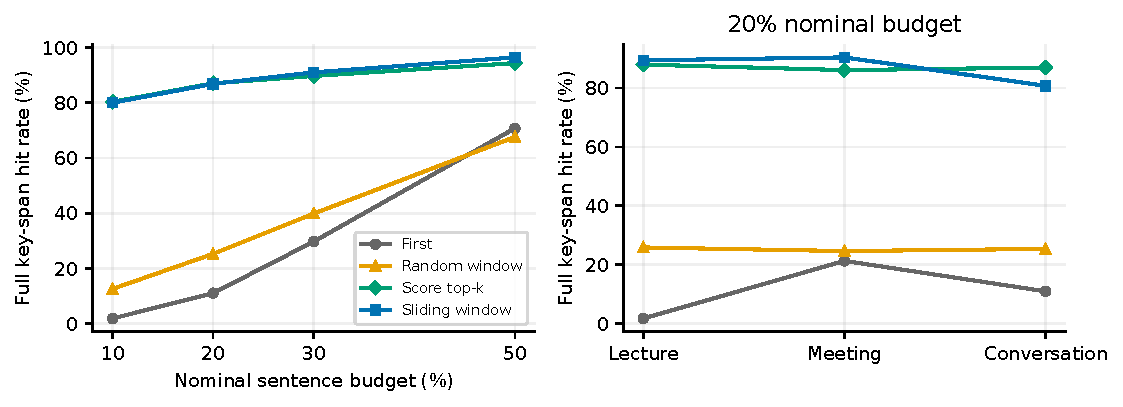
\includegraphics[width=0.94\textwidth]{retrieval.pdf}
\caption{左：完整关键跨度命中率随名义句数预算变化。右：20\% 预算下按场景分组的结果。所有方法共用 TF-IDF 分数；随机窗口为所有合法开始位置的精确期望。}
\label{fig:retrieval}
\end{figure*}

\subsection{连续性与场景差异}
20\% 预算下，滑动窗口在讲座、会议、日常对话上的命中率分别为 89.43\%、90.43\% 和 80.77\%；Top-$k$ 分别为 88.00\%、86.11\% 和 86.98\%。连续窗口在不同场景中的表现并不一致，尤其在日常对话上低于分散选择。

滑动窗口始终返回一个连续段，Top-$k$ 在该预算下平均返回 2.68 段。所选分数之和则分别为 0.7177 和 0.8924。后者更高符合其无连续性约束的选择目标，但分数更高并不保证完整跨度命中率在所有预算下都更高。图~\ref{fig:example} 展示按数据顺序预先指定的第一条记录，而非依据方法效果挑选的案例。

\begin{figure}[t]
\centering
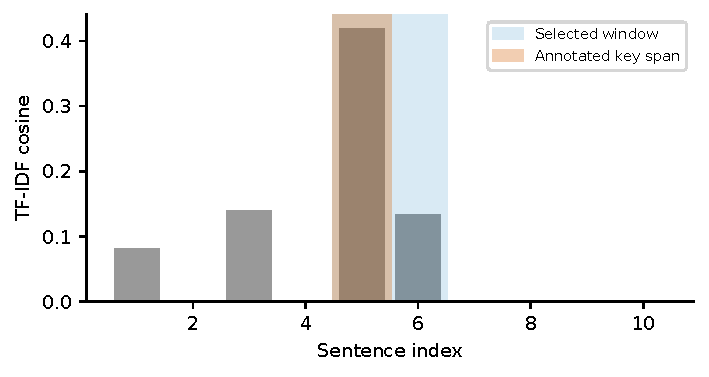
\includegraphics[width=\columnwidth]{example.pdf}
\caption{记录 \texttt{lecture\_0} 的句子分数、选中窗口与标注关键跨度，名义预算为 20\%。蓝色表示选择区间，橙色表示标注区间。}
\label{fig:example}
\end{figure}

\subsection{预算实际含义与标注敏感性}
由于向上取整，名义 20\% 预算对应的实际平均句数保留率为 22.47\%。该预算下，滑动窗口保留平均 25.25\% 的文本词数，Top-$k$ 为 28.25\%。因此，表中的同预算比较控制的是句子数量；句长差异仍会影响实际输入长度。

在 924 条标注文本完全一致的记录上，20\% 预算下的滑动窗口命中率为 86.90\%，Top-$k$ 为 87.23\%，随机窗口为 25.31\%。这一敏感性结果与全部记录上的主要排序接近，完整逐条标注审计随代码提供。

\subsection{正确性与选择开销}
2,000 个整数数组的最优窗口和与位置均与朴素扫描完全一致，4,048 个真实组合的窗口目标值均通过核对。长度 1,000、3,000、10,000 时，滑动更新的中位时间分别为 \SlideSmall、\SlideMedium、\SlideLarge 毫秒；朴素扫描分别为 \NaiveSmall、\NaiveMedium、\NaiveLarge 毫秒。计时在单台 Windows 11、Intel Family 6 Model 183 CPU 环境中完成，仅包含已生成分数后的选择调用。

计时结果与复杂度分析一致：当 $k=N/10$ 随输入增长时，朴素重复求和产生近似二次规模的工作量，而滑动更新保持线性扫描。这一比较解释的是窗口搜索的实现差异，语音转写和大模型推理的速度需在完整系统中另行测量。

\section{讨论与应用范围}
本文方案适合定位局部证据；相距较远的多处证据可能需要多个窗口。词语重合打分对同义改写和跨句推理的支持有限，可以用句向量或音频--文本对齐分数替换，再评价检索效果。

本文实证使用参考转写，未运行 ASR 或音频语言模型。映射回录音需要句子时间戳，固定秒数预算则应改用等时块或时间戳区间。端到端问答准确率、音频拼接效果和推理加速需要相应系统实验。

\section{结论}
本文基于 SpeechPrune 的问题背景，研究转写引导的连续片段选择，将其实现为固定长度最大和窗口搜索。循环不变式证明算法在已知分数下求得最优窗口，选择阶段为线性时间。在 1,012 条 SPIRAL 标注上，名义 20\% 句数预算下的完整关键跨度命中率为 86.86\%，并固定保留一个连续片段。不同预算与场景下相对于 Top-$k$ 的结果说明，连续性与证据覆盖需要联合评价。该案例以简单的打分、数组更新和可复现实验构成完整的算法课程研究。

\section*{复现与辅助工具说明}
公开标注下载脚本、窗口算法、四种比较方法、逐条结果、标注审计和绘图代码随项目提供。实验数值由程序实际计算。生成式人工智能参与了研究整理、代码与文字编写，提交者应完成个人复核并依据课程要求说明使用情况。
\bibliographystyle{IEEEtran}
\bibliography{references}
\end{document}
